% -*- Mode:TeX -*-

%% IMPORTANT: The official thesis specifications are available at:
%%            http://libraries.mit.edu/archives/thesis-specs/
%%
%%            Please verify your thesis' formatting and copyright
%%            assignment before submission.  If you notice any
%%            discrepancies between these templates and the 
%%            MIT Libraries' specs, please let us know
%%            by e-mailing thesis@mit.edu

%% The documentclass options along with the pagestyle can be used to generate
%% a technical report, a draft copy, or a regular thesis.  You may need to
%% re-specify the pagestyle after you \include  cover.tex.  For more
%% information, see the first few lines of mitthesis.cls. 

%\documentclass[12pt,vi,twoside]{mitthesis}
%%
%%  If you want your thesis copyright to you instead of MIT, use the
%%  ``vi'' option, as above.
%%
%\documentclass[12pt,twoside,leftblank]{mitthesis}
%%
%% If you want blank pages before new chapters to be labelled ``This
%% Page Intentionally Left Blank'', use the ``leftblank'' option, as
%% above. 

\documentclass[12pt,twoside]{mitthesis}
\usepackage{lgrind}

%% Packages not included in the template
\usepackage{import}
\usepackage{color}
\usepackage{graphicx}

%% These have been added at the request of the MIT Libraries, because
%% some PDF conversions mess up the ligatures.  -LB, 1/22/2014
\usepackage{cmap}
\usepackage[T1]{fontenc}
\pagestyle{plain}

%% This bit allows you to either specify only the files which you wish to
%% process, or `all' to process all files which you \include.
%% Krishna Sethuraman (1990).

\typein [\files]{Enter file names to process, (chap1,chap2 ...), or `all' to
process all files:}
\def\all{all}
\ifx\files\all \typeout{Including all files.} \else \typeout{Including only \files.} \includeonly{\files} \fi

\begin{document}

% -*-latex-*-
% 
% For questions, comments, concerns or complaints:
% thesis@mit.edu
% 
%
% $Log: cover.tex,v $
% Revision 1.8  2008/05/13 15:02:15  jdreed
% Degree month is June, not May.  Added note about prevdegrees.
% Arthur Smith's title updated
%
% Revision 1.7  2001/02/08 18:53:16  boojum
% changed some \newpages to \cleardoublepages
%
% Revision 1.6  1999/10/21 14:49:31  boojum
% changed comment referring to documentstyle
%
% Revision 1.5  1999/10/21 14:39:04  boojum
% *** empty log message ***
%
% Revision 1.4  1997/04/18  17:54:10  othomas
% added page numbers on abstract and cover, and made 1 abstract
% page the default rather than 2.  (anne hunter tells me this
% is the new institute standard.)
%
% Revision 1.4  1997/04/18  17:54:10  othomas
% added page numbers on abstract and cover, and made 1 abstract
% page the default rather than 2.  (anne hunter tells me this
% is the new institute standard.)
%
% Revision 1.3  93/05/17  17:06:29  starflt
% Added acknowledgements section (suggested by tompalka)
% 
% Revision 1.2  92/04/22  13:13:13  epeisach
% Fixes for 1991 course 6 requirements
% Phrase "and to grant others the right to do so" has been added to 
% permission clause
% Second copy of abstract is not counted as separate pages so numbering works
% out
% 
% Revision 1.1  92/04/22  13:08:20  epeisach

% NOTE:
% These templates make an effort to conform to the MIT Thesis specifications,
% however the specifications can change.  We recommend that you verify the
% layout of your title page with your thesis advisor and/or the MIT 
% Libraries before printing your final copy.
\title{A 64 Channel 3T Array Coil for Highly Accelerated Fetal Imaging at 22 Weeks of Pregnancy}

\author{Mark H. Spatz}
% If you wish to list your previous degrees on the cover page, use the 
% previous degrees command:
%       \prevdegrees{A.A., Harvard University (1985)}
% You can use the \\ command to list multiple previous degrees
%       \prevdegrees{B.S., University of California (1978) \\
%                    S.M., Massachusetts Institute of Technology (1981)}
\department{Department of Electrical Engineering and Computer Science}

% If the thesis is for two degrees simultaneously, list them both
% separated by \and like this:
% \degree{Doctor of Philosophy \and Master of Science}
\degree{Master of Engineering in Electrical Engineering and Computer Science}

% As of the 2007-08 academic year, valid degree months are September, 
% February, or June.  The default is June.
\degreemonth{February}
\degreeyear{2017}
\thesisdate{Feb 3, 2017}

%% By default, the thesis will be copyrighted to MIT.  If you need to copyright
%% the thesis to yourself, just specify the `vi' documentclass option.  If for
%% some reason you want to exactly specify the copyright notice text, you can
%% use the \copyrightnoticetext command.  
%\copyrightnoticetext{\copyright IBM, 1990.  Do not open till Xmas.}

% If there is more than one supervisor, use the \supervisor command
% once for each.
\supervisor{Lawrence L. Wald}{Professor of Radiology, Harvard Medical School}

% This is the department committee chairman, not the thesis committee
% chairman.  You should replace this with your Department's Committee
% Chairman.
\chairman{Christopher Terman}{Chairman, Masters of Engineering Thesis Committee}

% Make the titlepage based on the above information.  If you need
% something special and can't use the standard form, you can specify
% the exact text of the titlepage yourself.  Put it in a titlepage
% environment and leave blank lines where you want vertical space.
% The spaces will be adjusted to fill the entire page.  The dotted
% lines for the signatures are made with the \signature command.
\maketitle

% The abstractpage environment sets up everything on the page except
% the text itself.  The title and other header material are put at the
% top of the page, and the supervisors are listed at the bottom.  A
% new page is begun both before and after.  Of course, an abstract may
% be more than one page itself.  If you need more control over the
% format of the page, you can use the abstract environment, which puts
% the word "Abstract" at the beginning and single spaces its text.

%% You can either \input (*not* \include) your abstract file, or you can put
%% the text of the abstract directly between the \begin{abstractpage} and
%% \end{abstractpage} commands.

% First copy: start a new page, and save the page number.
\cleardoublepage
% Uncomment the next line if you do NOT want a page number on your
% abstract and acknowledgments pages.
% \pagestyle{empty}
\setcounter{savepage}{\thepage}
\begin{abstractpage}
% $Log: abstract.tex,v $
% Revision 1.1  93/05/14  14:56:25  starflt
% Initial revision
% 
% Revision 1.1  90/05/04  10:41:01  lwvanels
% Initial revision
% 
%
%% The text of your abstract and nothing else (other than comments) goes here.
%% It will be single-spaced and the rest of the text that is supposed to go on
%% the abstract page will be generated by the abstractpage environment.  This
%% file should be \input (not \include 'd) from cover.tex.
In this thesis, I designed and implemented a compiler which performs
optimizations that reduce the number of low-level floating point operations
necessary for a specific task; this involves the optimization of chains of
floating point operations as well as the implementation of a ``fixed'' point
data type that allows some floating point operations to simulated with integer
arithmetic.  The source language of the compiler is a subset of C, and the
destination language is assembly language for a micro-floating point CPU.  An
instruction-level simulator of the CPU was written to allow testing of the
code.  A series of test pieces of codes was compiled, both with and without
optimization, to determine how effective these optimizations were.

\end{abstractpage}

% Additional copy: start a new page, and reset the page number.  This way,
% the second copy of the abstract is not counted as separate pages.
% Uncomment the next 6 lines if you need two copies of the abstract
% page.
% \setcounter{page}{\thesavepage}
% \begin{abstractpage}
% % $Log: abstract.tex,v $
% Revision 1.1  93/05/14  14:56:25  starflt
% Initial revision
% 
% Revision 1.1  90/05/04  10:41:01  lwvanels
% Initial revision
% 
%
%% The text of your abstract and nothing else (other than comments) goes here.
%% It will be single-spaced and the rest of the text that is supposed to go on
%% the abstract page will be generated by the abstractpage environment.  This
%% file should be \input (not \include 'd) from cover.tex.
In this thesis, I designed and implemented a compiler which performs
optimizations that reduce the number of low-level floating point operations
necessary for a specific task; this involves the optimization of chains of
floating point operations as well as the implementation of a ``fixed'' point
data type that allows some floating point operations to simulated with integer
arithmetic.  The source language of the compiler is a subset of C, and the
destination language is assembly language for a micro-floating point CPU.  An
instruction-level simulator of the CPU was written to allow testing of the
code.  A series of test pieces of codes was compiled, both with and without
optimization, to determine how effective these optimizations were.

% \end{abstractpage}

\cleardoublepage

\section*{Acknowledgments}

This is the acknowledgements section.  You should replace this with your
own acknowledgements.

%%%%%%%%%%%%%%%%%%%%%%%%%%%%%%%%%%%%%%%%%%%%%%%%%%%%%%%%%%%%%%%%%%%%%%
% -*-latex-*-

% Some departments (e.g. 5) require an additional signature page.  See
% signature.tex for more information and uncomment the following line if
% applicable.
% % -*- Mode:TeX -*-
%
% Some departments (e.g. Chemistry) require an additional cover page
% with signatures of the thesis committee.  Please check with your
% thesis advisor or other appropriate person to determine if such a 
% page is required for your thesis.  
%
% If you choose not to use the "titlepage" environment, a \newpage
% commands, and several \vspace{\fill} commands may be necessary to
% achieve the required spacing.  The \signature command is defined in
% the "mitthesis" class
%
% The following sample appears courtesy of Ben Kaduk <kaduk@mit.edu> and
% was used in his June 2012 doctoral thesis in Chemistry. 

\begin{titlepage}
\begin{large}
This doctoral thesis has been examined by a Committee of the Department
of Chemistry as follows:

\signature{Professor Jianshu Cao}{Chairman, Thesis Committee \\
   Professor of Chemistry}

\signature{Professor Troy Van Voorhis}{Thesis Supervisor \\
   Associate Professor of Chemistry}

\signature{Professor Robert W. Field}{Member, Thesis Committee \\
   Haslam and Dewey Professor of Chemistry}
\end{large}
\end{titlepage}


\pagestyle{plain}
  % -*- Mode:TeX -*-
%% This file simply contains the commands that actually generate the table of
%% contents and lists of figures and tables.  You can omit any or all of
%% these files by simply taking out the appropriate command.  For more
%% information on these files, see appendix C.3.3 of the LaTeX manual. 
\tableofcontents
\newpage
\listoffigures
\newpage
\listoftables


\chapter{Loop Elements}

The same basic loop circuit, shown in figure \ref{fig:loop_schematic}, is duplicated 64 times to create the full array.
Here, I will discuss the purpose and function of each part of this circuit.

\section{Active Detuning}
The loop is a resonant circuit that is strongly coupled to the volume surrounding it. It is necessary to spoil this
resonance during the high power RF transmit pulses so that excessive currents are not induced in the loop. Such
unintended energy deposition could adversely affect transmit homogenaity, damage the array, or create a safety hazard.
This selective detuning is acheived by switching an inductor across one of the loop capacitors, creating a parallel
resonant tank that behaves as an open circuit in the loop at $\omega_L$.

A DC bias current of about $120mA$ is injected on the line marked BIAS in figure \ref{fig:loop_schematic}. This bias
current flows through a PIN diode, $D_1$, creating an RF short and effectively switching $L_{TRAP}$ across $C_{S3}$.
$L_{TRAP}$ is an adjustable air core inductor, and is hand tuned to resonate with $C_{S3}$ at precisely $\omega_L$. The 
parallel resonant circuit thus formed creates a virtual open ciruit in the loop, preventing current from flowing. As 
soon as the bias current is removed and the diode recovers, the trap is disabled and the loop once again becomes tuned.

\section{Passive Detuning}
The active detuning strategy is sufficient for assurance of image quality and protection from hardware damage, but a
passive method is required to ensure patient safety in the event of an electrical failure. The crossed diode pair $D_2$
clamps the voltage across $C_{S3}$ and $L_{TRAP}$ to safe levels, passively enabling the trap if the energy stored in
the loop gets too high. Other designs might also include RF fuses in the loop circuit, but the loops employed in this
array are all small enough that this was not necesarry.

\begin{figure}
    \centering
    \input{figures/loop_diagram.pdf_tex}
    \caption{Complete loop circuit schematic}
    \label{fig:loop_schematic}
\end{figure}

\section{Loop Model}
The essence of the wire loop receive elements used in this array is a damped series resonant circuit, shown in figure
\ref{fig:loop_model} A. The loop has a distributed inductance by nature of its geometry, and is broken at regular
intervals by discrete capacitors.  Wire and component resistances and (more importantly) inductive coupling to adjacent
conductive materials reduces the loop Q to a finite value. This effect is modelled by a series resistor with value
$R_{LOAD}=\sqrt{\frac{L}{C}}\cdot\frac{1}{Q}$

\section{Loop Circuit Output port}
Figure \ref{fig:loop_model} B shows the creation of an output port in the loop circuit. The total loop capacitance is
split into $C_P$, across which the output port is formed, and $C_S$. A series capacitor $C_M$ is added to one terminal
of the output port.

%For the purpose of further analisys, it is convenient to lump component impedances together into
%#three blocks: $Z_P$ (parallel imedance), $Z_S$ (series impedance), and $Z_M$ (matching impedance). These impedances are
%#defined in figure \ref{fig:loop_model} C.

\begin{figure}
    \centering
    \input{figures/loop_model.pdf_tex}
    \caption{Loop circuit models}
    \label{fig:loop_model}
\end{figure}

\section{Loop Circuit Analisys}
The loop ciruit has an input inpedance of $Z_{IN}$ at its port, as defined in equation \ref{eq:Z_IN}. This impedance can
be split into its real and imaginary parts, $R_{IN}$ and $X_{IN}$, shown in equations \ref{eq:R_IN} and \ref{eq:X_IN}.

\begin{equation} \label{eq:Z_IN}
    Z_{IN}=(jX_p)\parallel(jX_S+R_{L})+jX_M = \frac{1}{j\omega \cdot C_P + \frac{1}{R_{L}+j\omega\cdot L_{L} +
    \frac{1}{j\omega \cdot C_S}}} + \frac{1}{j\omega\cdot C_M}
\end{equation}

\begin{equation} \label{eq:R_IN}
    R_{IN}=\frac{{C_S}^2 R_{L}}{{C_P}^2 {C_S}^2 {L_{LOOP}}^2 \omega^4 + {C_P}^2 {C_S}^2 {R_{L}}^2
    \omega^2 - 2 {C_P}^2 C_S L_{L} \omega^2 + {C_P}^2 - 2 C_P {C_S}^2 L_{L} \omega^2 + 2 C_P C_S + {C_S}^2}
\end{equation}

\begin{equation} \label{eq:X_IN}
    X_{IN}= Im(Z_{IN}) = \frac{X_P ({R_L}^2 + X_S(X_P+X_S))}{{R_L}^2+(X_P+X_S)^2}+X_M
\end{equation}

\section{Loop Component selection}

\subsection{Loop Circuit Considerations}
\subsubsection{Minimizing Preamp Noise Figure}
The vendor supplied preamplifier is designed to achieve minimum noise figure when presented with a purely real
$50\Omega$ load at its input. Therefore, component values should be selected such that $R_{IN}=50\Omega$ and
$X_{IN}=0\Omega$. Call this optimal input impedance $Z_{IN_{OPT}}$.

\subsubsection{Preamp Decoupling}
Preamp decoupling is typicall achieved by resonating a capacitor in the loop ($C_P$ in figure \ref{fig:loop_model}) with
an inductor in series with one terminal of the output port (in the same position as $C_M$ in figure
\ref{fig:loop_model}) through the input of the preamplifier. In our case, however, the inductance is integrated into the
preamplifier itself. I measure the inductance of the preamplifer input to be roughly $130nH$ at $123.25 MHz$. The
details of the preamp topology are unavailible to me. I simply consider it to have an impedance of $Z_P$, which
is transformed to ${Z_P}'$ (as shown in equation \ref{eq:Z_PREAMP}) by the short length of coaxial cable (with
characteristic impeance $Z_0$) connecting the preamp to the loop.

\begin{equation} \label{eq:Z_PREAMP}
    {Z_P}'=Z_0 \cdot \frac{Z_P-j Z_0 \cdot \tan(2\pi\cdot\frac{L_{COAX}}{\lambda})}{Z_0 - j Z_P \cdot
    \tan(2\pi\cdot\frac{L_{COAX}}{\lambda})}
\end{equation}

\begin{equation} \label{eq:X_PREAMP}
    {X_P}'=Im({Z_P}')
\end{equation}
    
In any case, preamp decoupling is achieved when $C_P$, $C_M$, and the transformed preamp input impedance resonate
together, as defined in equation \ref{eq:preamp_decoupling_condition}.

\begin{equation} \label{eq:preamp_decoupling_condition}
    X_P + X_M +{X_P}' = 0
\end{equation}


\subsection{Loop Resonance}

I define loop resonance as occuring at a frequency $\omega_0$ where $X_P + X_S = 0$. In this case, the equations for
$R_{IN}$ and $X_{IN}$ simplify to equations \ref{eq:R_IN_RES} and \ref{eq:X_IN_RES} respectively. Rearranging equation
\ref{eq:R_IN_RES} into equation \ref{eq:X_P_RIN} gives a formula for setting the value of $R_IN$ on resonance; however,
it is then impossible to select $X_M$ to simultaneously achieve zero $X_{IN}$ and satisfy the preamp decoupling conditon
(equation \ref{eq:preamp_decoupling_condition})


\begin{equation} \label{eq:R_IN_RES}
    R_{IN}\big|_{\omega=\omega_0}=\frac{{X_P}^2}{R_L} = \frac{{X_S}^2}{R_L} 
\end{equation}

\begin{equation} \label{eq:X_IN_RES}
    X_{IN}\big|_{\omega=\omega_0}=X_P+X_M=-X_S+X_M
\end{equation}

\begin{equation} \label{eq:X_P_RIN}
    X_{P}(R_{IN})\big|_{\omega=\omega_0}=-\sqrt{R_{LOAD} \cdot R_{IN}} 
\end{equation}

\subsection{Off resonance behavior}
It is not necessary that the loop be tuned to resonate precisely at the frequency of interest. The position of
$\omega_0$ relative to that of the Lamor frequency $\omega_L$ is another variable that we can manipulate to achieve the
desired loop circuit characteristics.

\subsubsection{Choosing $X_P$}
Consider choosing $X_P=-\sqrt{\alpha\ \cdot Z_{OPT} \cdot R_{LOAD}}$, so that the value of $R_{IN}$ on resonance is a
factor of $\alpha$ larger than $Z_{OPT}$. Substituting this value into eq. \ref{eq:R_IN}, we get a new equation for
$R_{IN}$: eq. \ref{eq:R_IN_alpha}. The frequency dependent value of $R_{IN}$ is plotted in figure
\ref{fig:impedance_plot}

\begin{equation} \label{eq:R_IN_alpha}
    R_{IN}\big|_{X_P=-\sqrt{\alpha Z_{OPT} R_{LOAD}}} = \frac{\alpha Z_{OPT} {R_{LOAD}}^2}{{R_L}^2 + \alpha Z_{OPT} R_{LOAD} - 2\sqrt{\alpha Z_{OPT} R_{LOAD}} X_S + {X_S}^2}
\end{equation}

\subsubsection{Choosing $X_S$}
Indeed, when $X_P=-\sqrt{\alpha Z_{OPT} R_{LOAD}}$ and $X_S=\sqrt{\alpha Z_{OPT} R_{LOAD}}$, eq.  \ref{eq:R_IN_alpha}
reduces to $R_{IN} = \alpha \cdot Z_{OPT}$.  But on either side of this resonant peak, there is a single frequency at
which $R_{IN} = Z_{OPT}$. Solving \ref{eq:R_IN_alpha} for the two values of $X_S$ at which this occurs, we get: $$X_S =
\sqrt{\alpha Z_{OPT} R_{LOAD}} \pm R_{LOAD} \sqrt{\alpha - 1}$$ We choose the minus sign in this expression, and thus
achieve $R_{IN} = Z_{OPT}$ at a frequency below $\omega_0$, because this makes the sytem of equations in the next step
solvable.

\subsubsection{Choosing $\alpha$ and $X_M$}
The only remaining free parameters are $\alpha$ and $X_M$.  They must be chosen to achieve purely real input inpedance
($X_{IN} = 0$) and preamp decoupling ($X_P + X_M +{X_P}' = 0$). Plugging in the values of $X_P$ and $X_S$ that we've
selected so far into these two requirements, we get a system of equations with a singe set of solutions:
$$
\begin{aligned}
    Z_{OPT} \sqrt{\alpha - 1} - \sqrt{\alpha Z_{OPT} R_{LOAD}} + X_M &= 0\\
    -\sqrt{\alpha Z_{OPT}} + X_M + {X_P}' &= 0
\end{aligned}
\implies
\begin{aligned}
    \alpha &= 1 + \frac{{X_P}'^2}{Z_{OPT}}\\
    X_M &= \sqrt{\frac{R_{LOAD}}{Z_{OPT}} ({X_P}'^2 + {Z_{OPT}}^2} - {X_P}'
\end{aligned}
$$

\subsection{Optimal Component values}



\begin{figure}
    \centering
    \input{figures/impedance_plot.pdf_tex}
    \caption{Loop impedances vs. frequency with optimal component values}
    \label{fig:impedance_plot}
\end{figure}

\appendix
\chapter{Tables}

\begin{table}
\caption{Armadillos}
\label{arm:table}
\begin{center}
\begin{tabular}{||l|l||}\hline
Armadillos & are \\\hline
our	   & friends \\\hline
\end{tabular}
\end{center}
\end{table}

\clearpage
\newpage

\chapter{Figures}

\vspace*{-3in}


\begin{figure}
\vspace{2.4in}
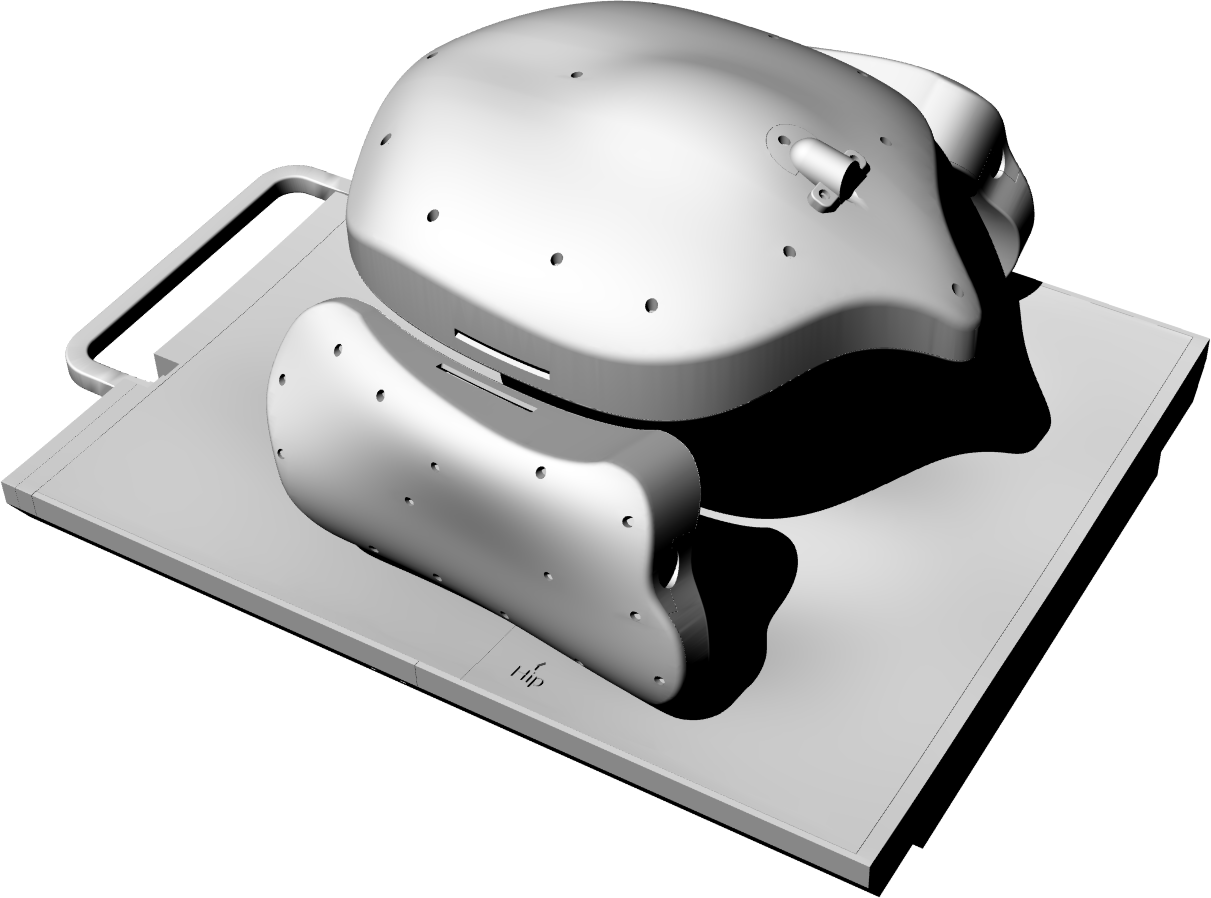
\includegraphics[width=6in]{figures/cad_rendering.png}
\caption{Computer rendering of array panels and housings}
\label{fig:cad_rendering}
\end{figure}
\clearpage
\newpage

\begin{figure}
\vspace{2.4in}
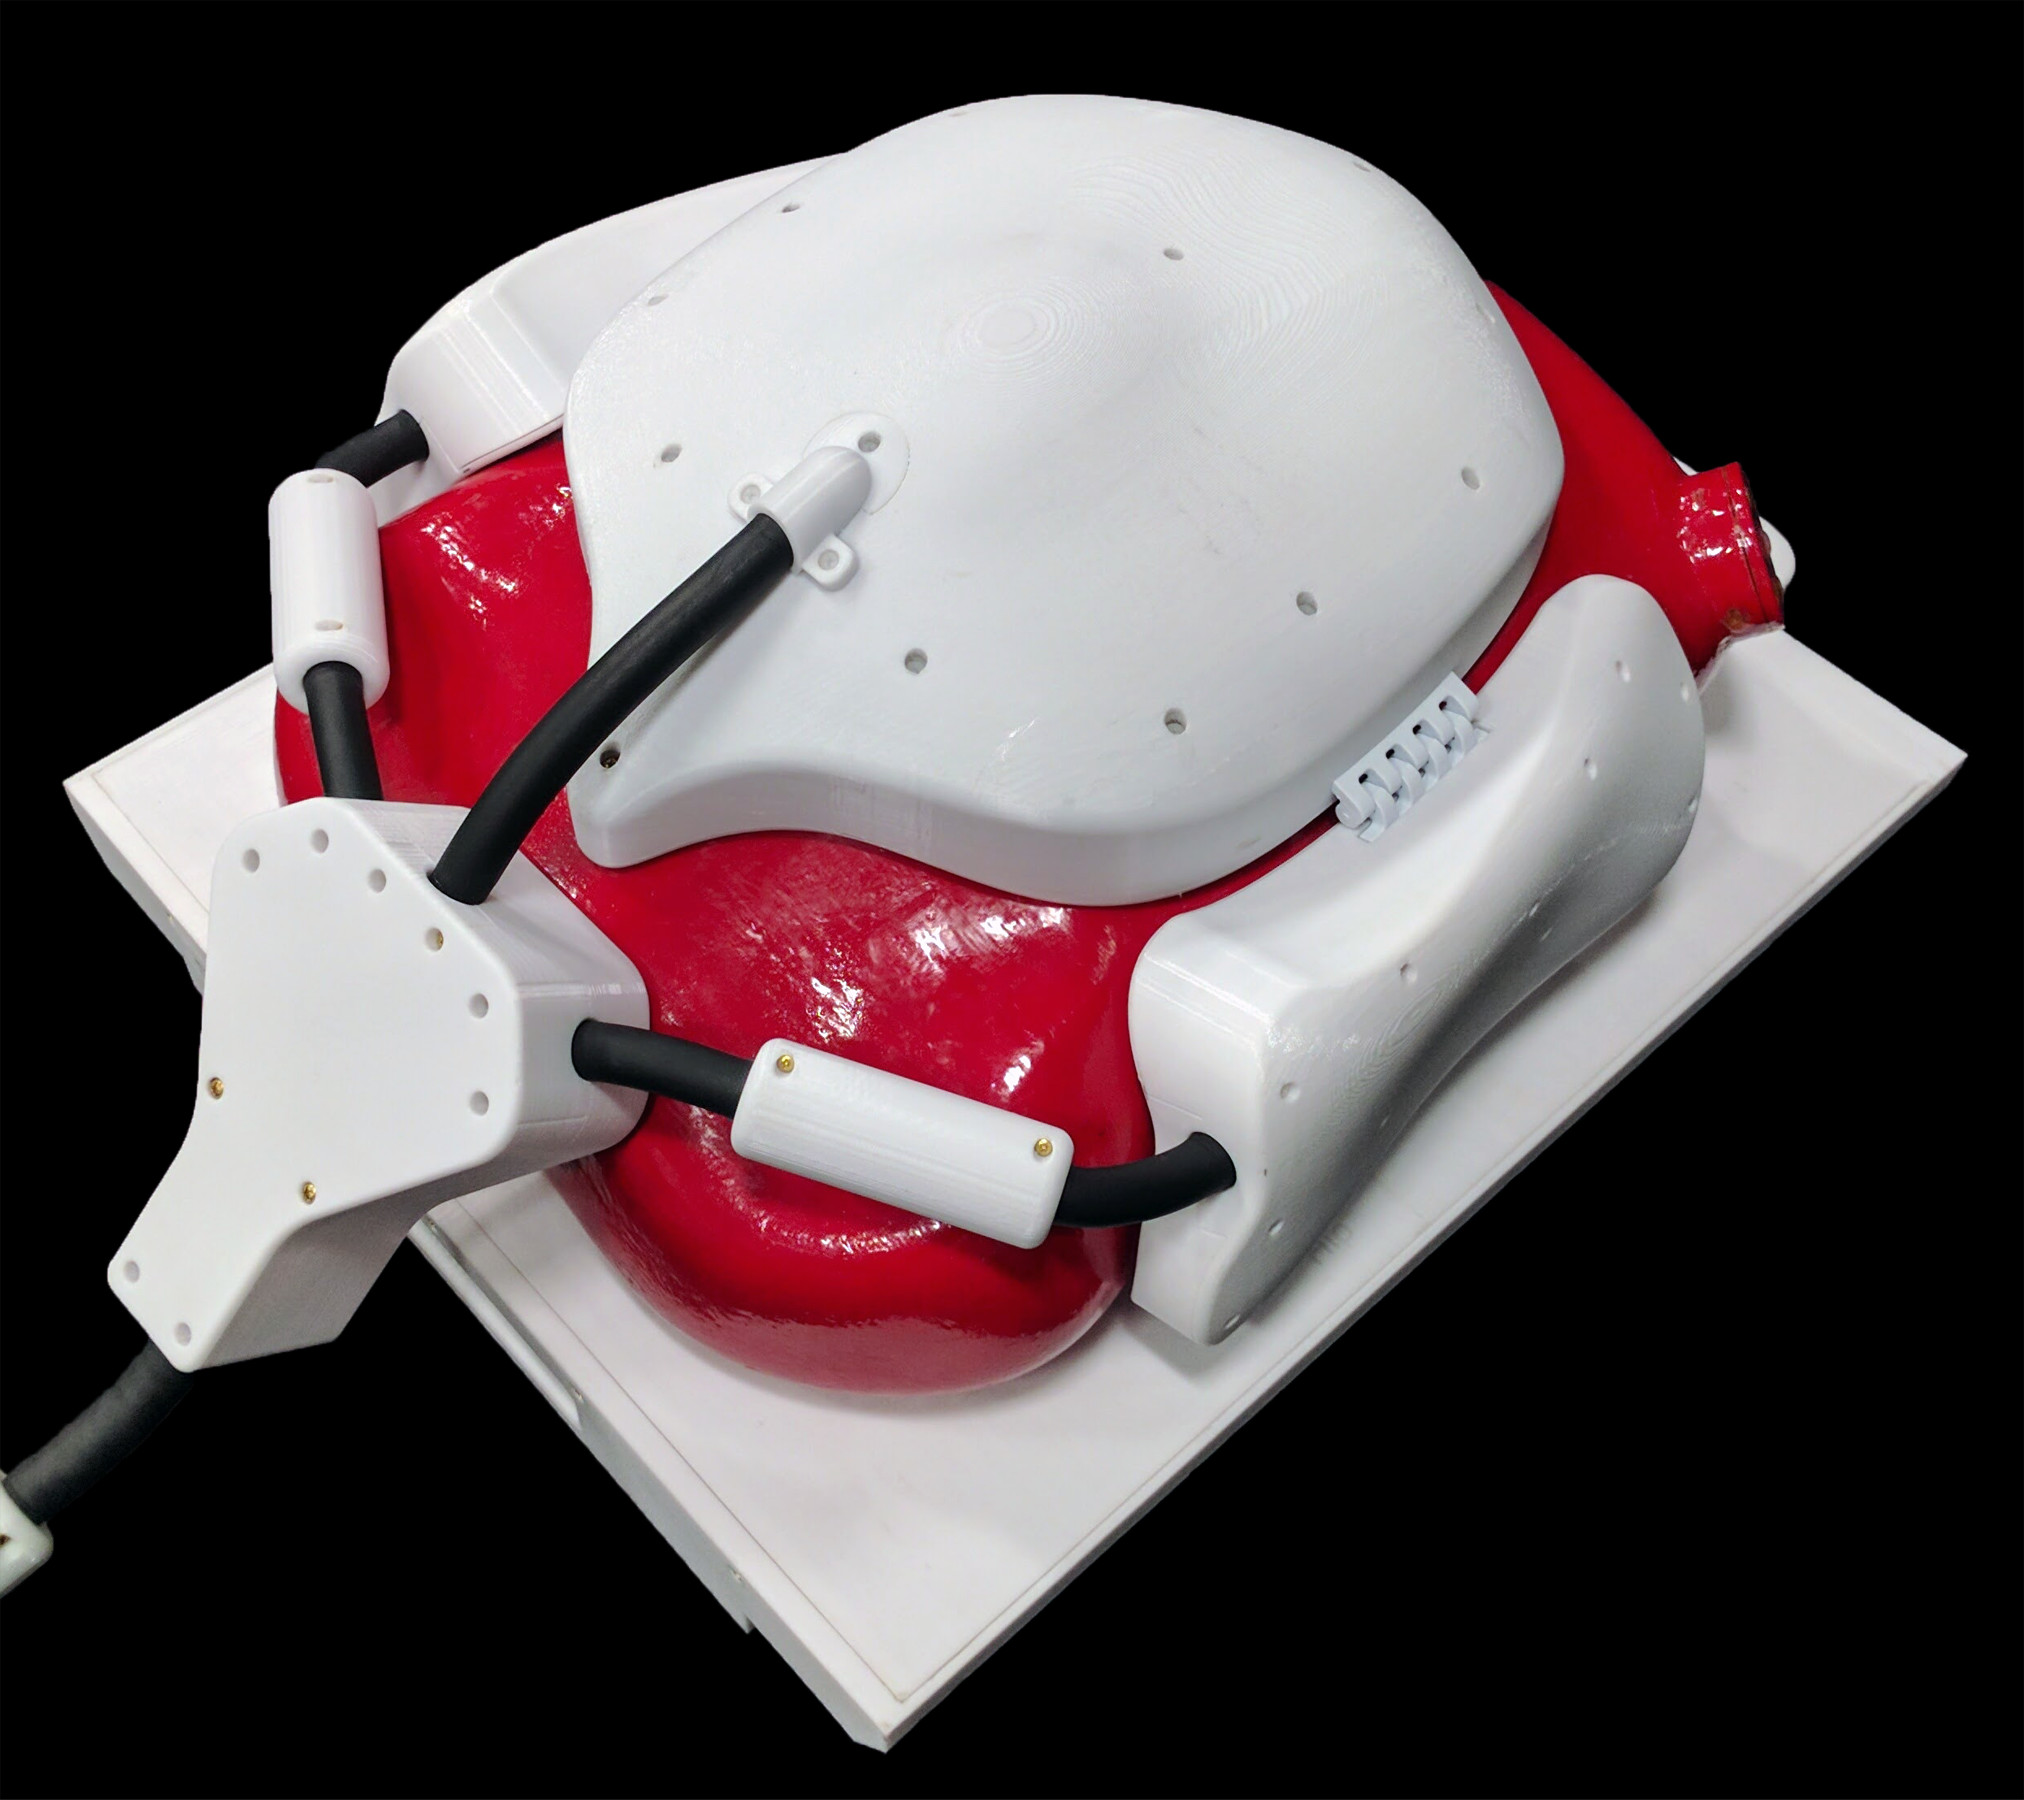
\includegraphics[width=6in]{figures/assembled_view.jpg}
\caption{Finished coil, posed on 22 week pregnant abdomen phantom}
\label{fig:assembled_view}
\end{figure}
\clearpage
\newpage

\begin{figure}
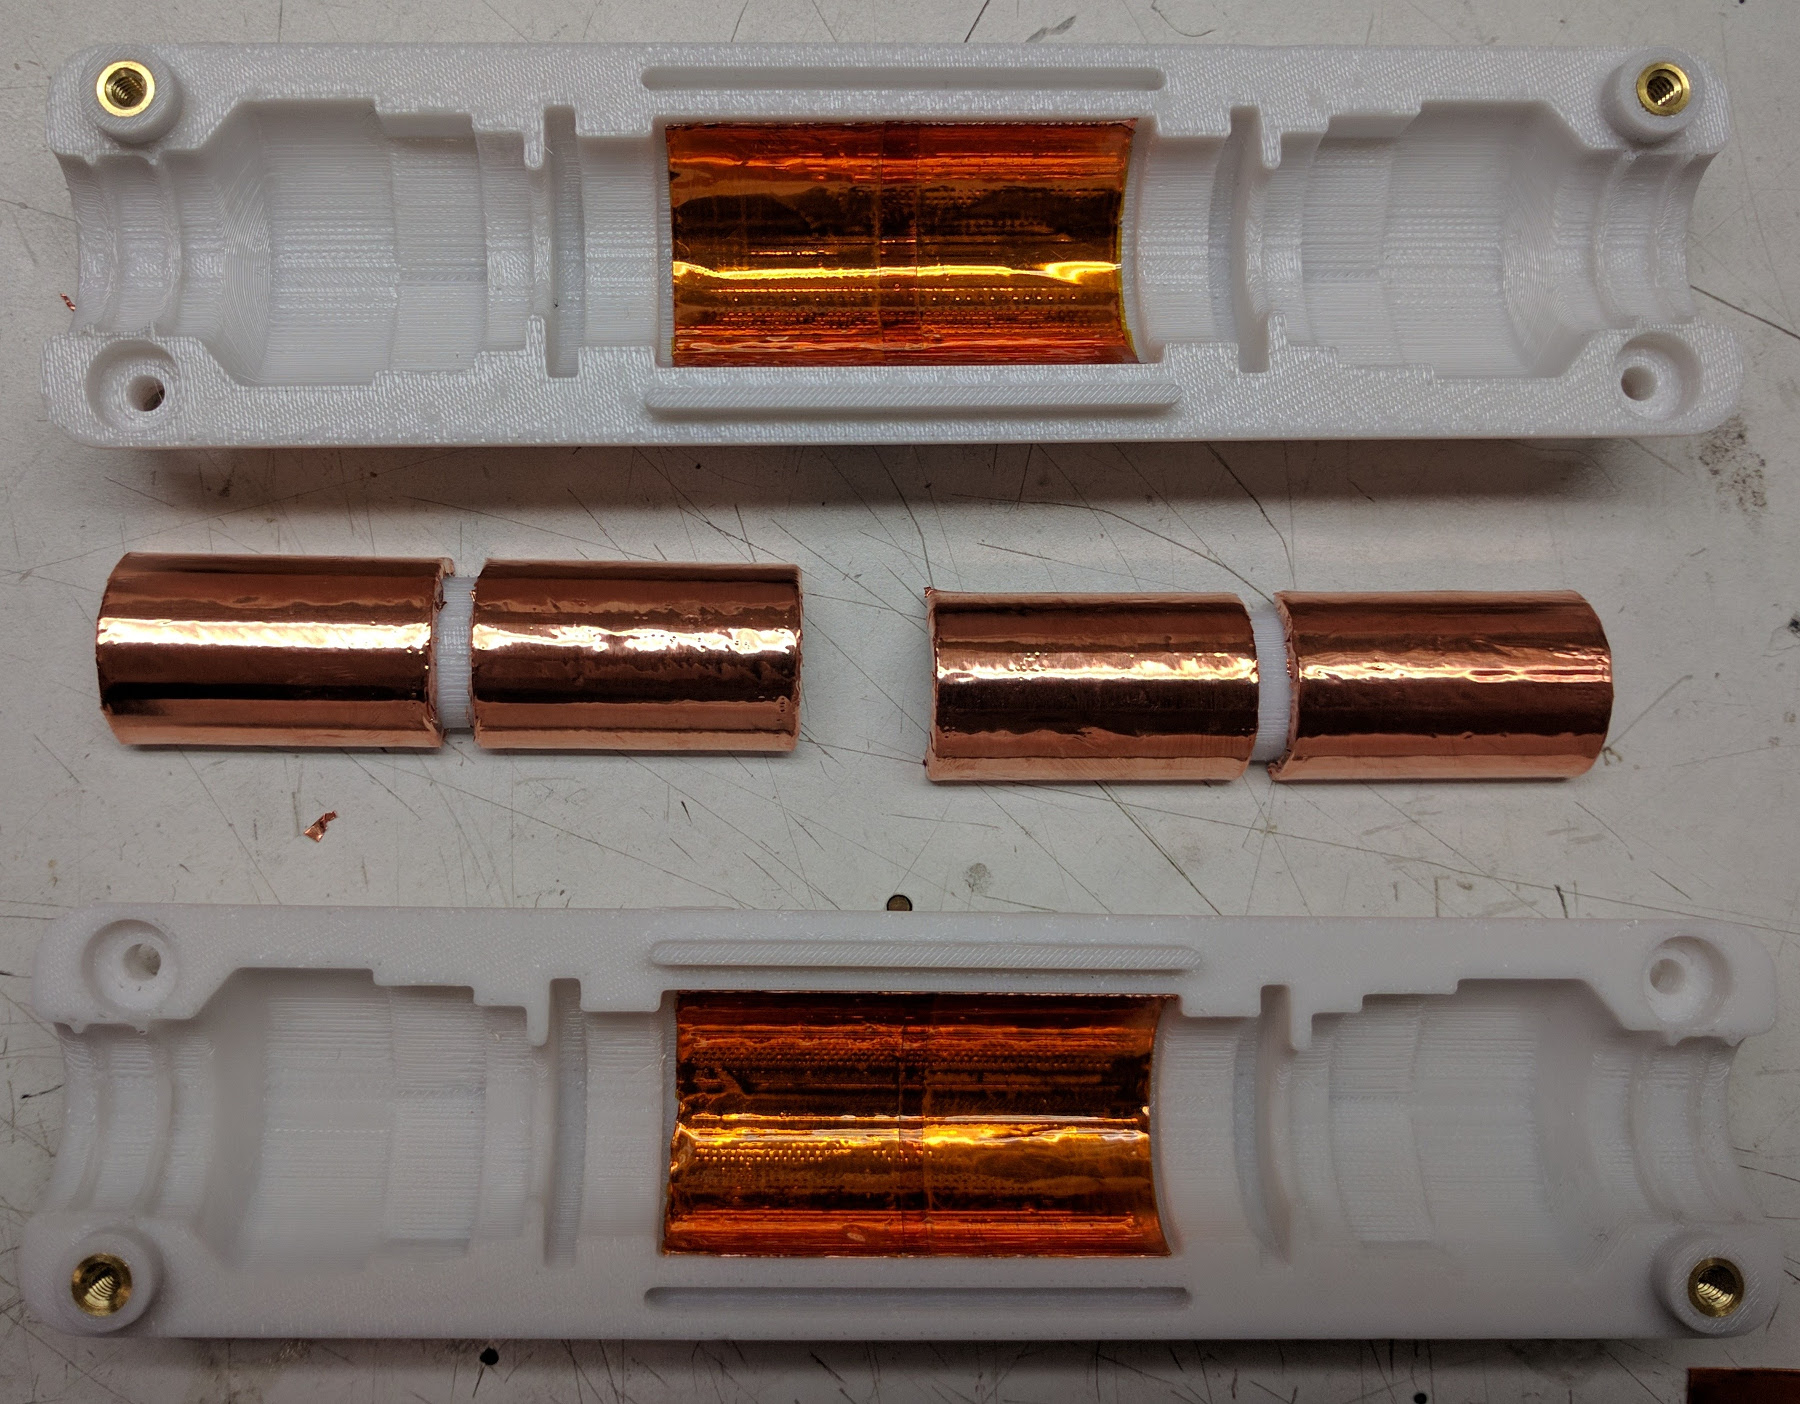
\includegraphics[width=6in]{figures/bazooka_parts.jpg}
\caption{Bazooka Balun before assembly}
\label{fig:bazooka_parts}
\end{figure}

\begin{figure}
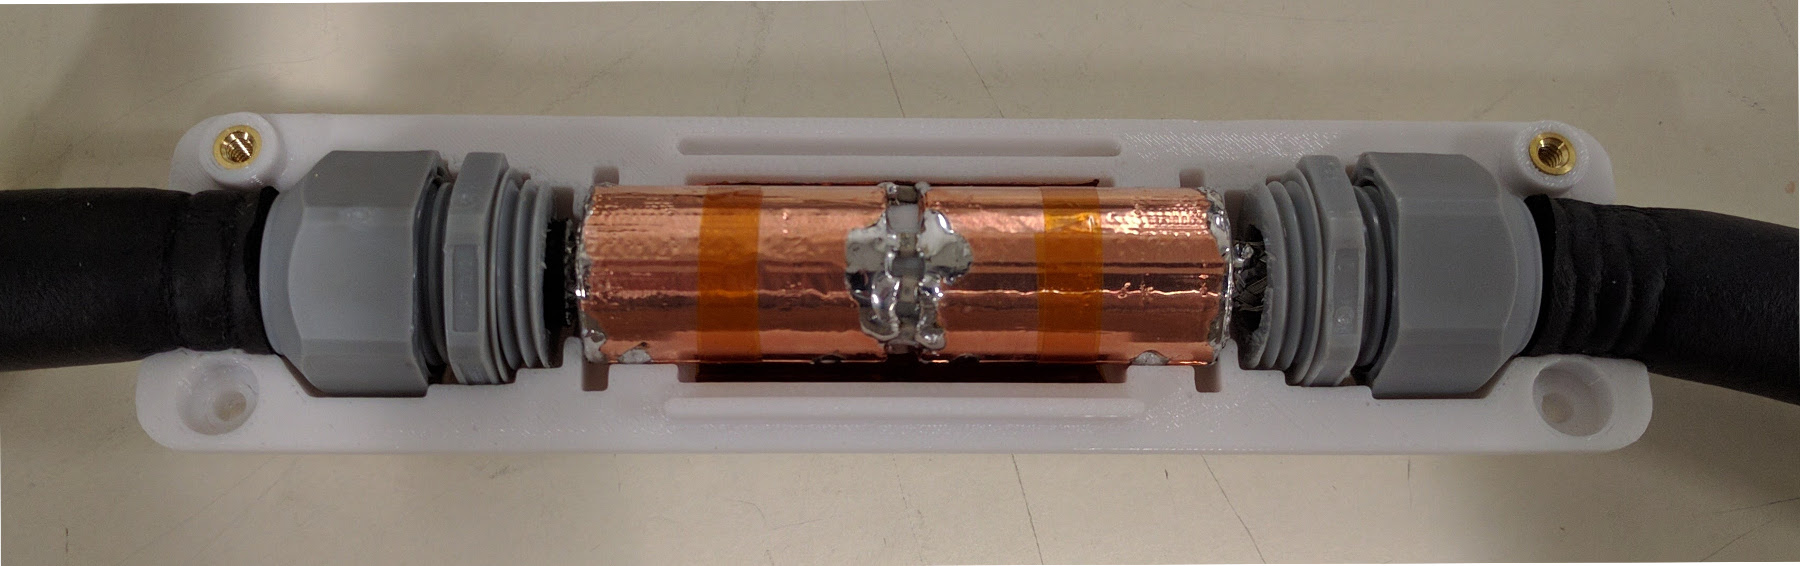
\includegraphics[width=6in]{figures/bazooka_assembled.jpg}
\caption{Completed bazooka balun with open enclosure}
\label{fig:bazooka_assembled}
\end{figure}
\clearpage
\newpage

\begin{figure}
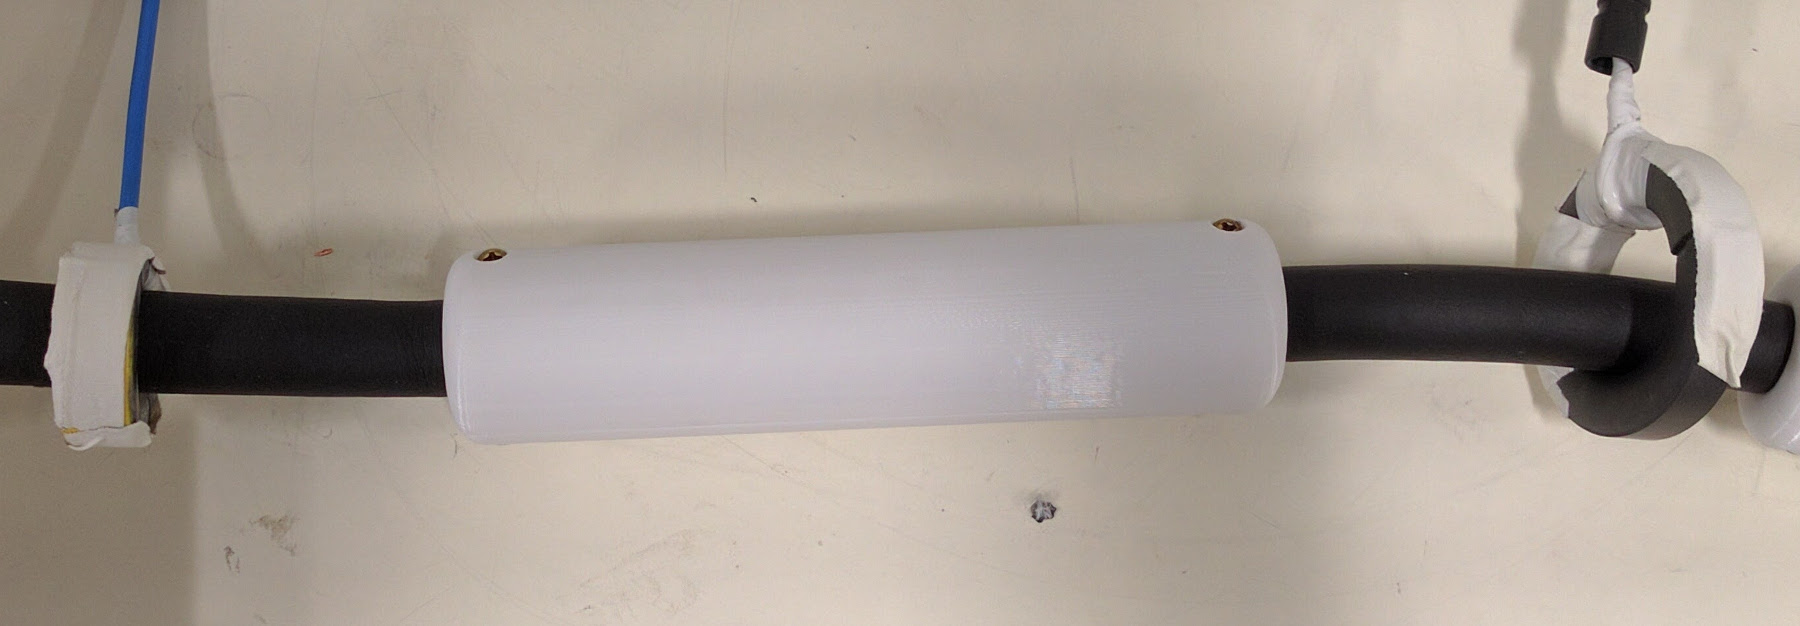
\includegraphics[width=6in]{figures/bazooka_under_test.jpg}
\caption{Cable trap with current injection probes}
\label{fig:bazooka_under_test}
\end{figure}
\clearpage
\newpage

\begin{figure}
\vspace{2.4in}
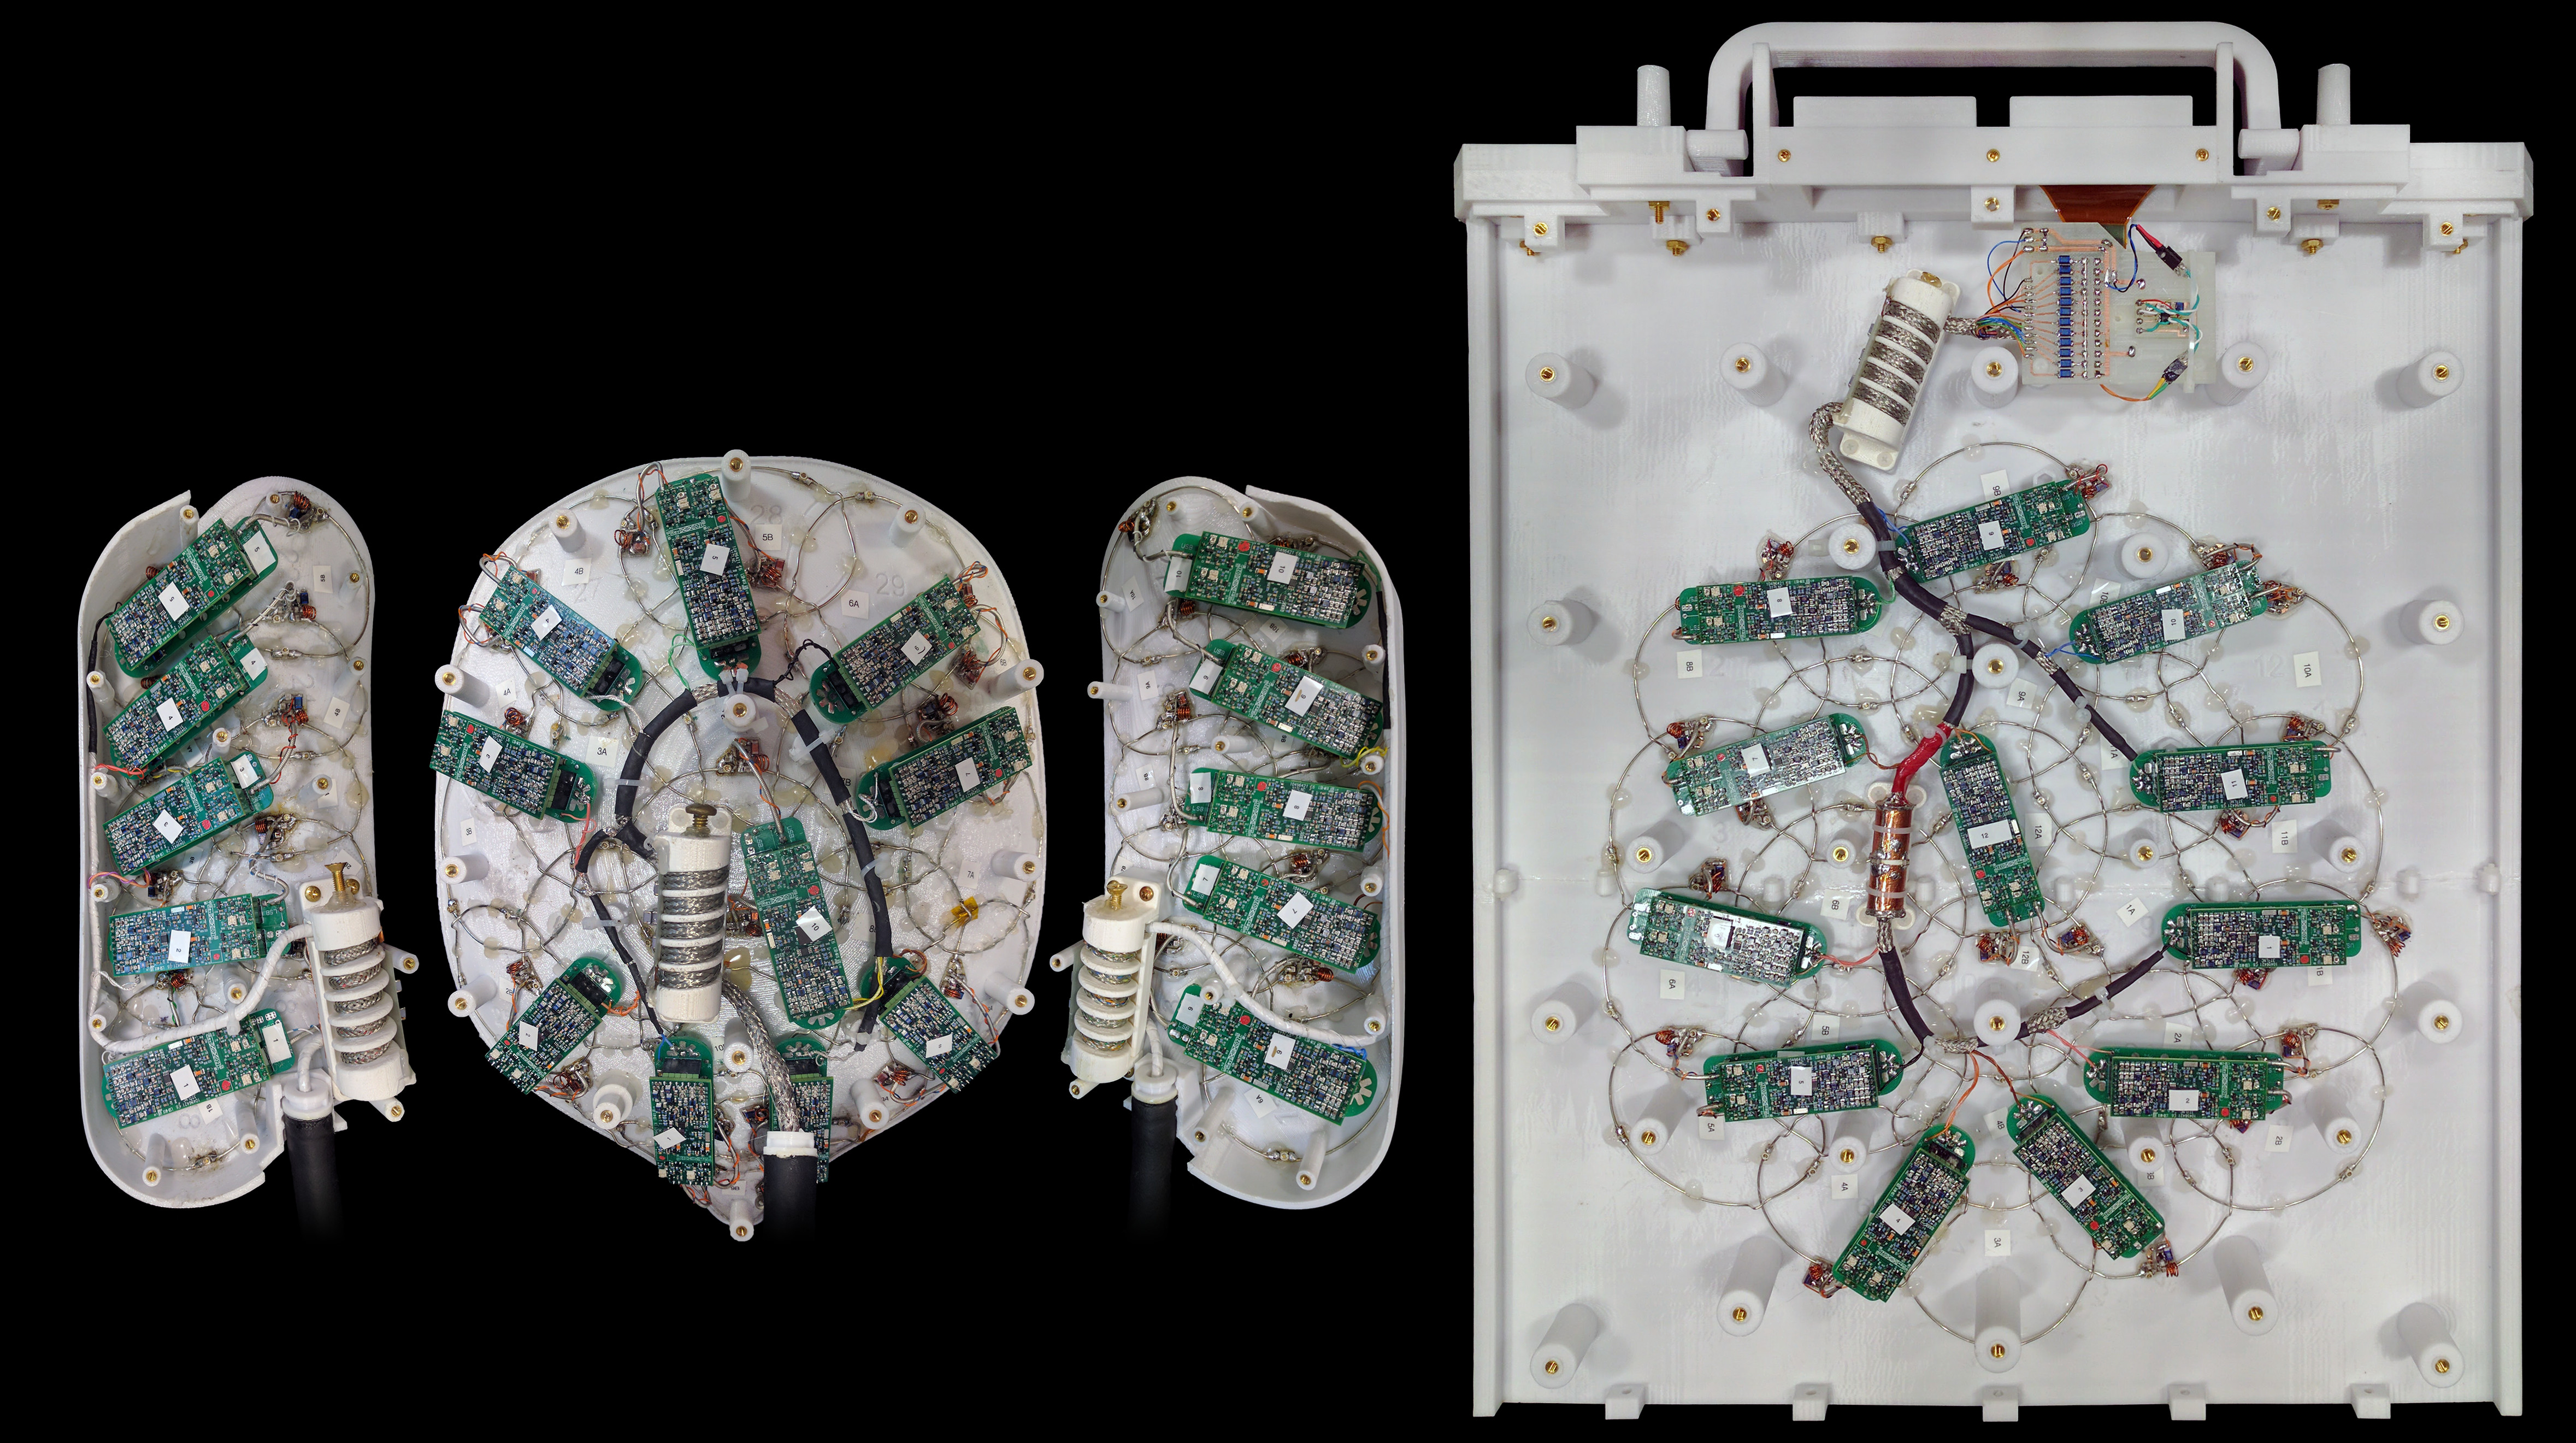
\includegraphics[width=6in]{figures/internals_composite.jpg}
\caption{View of internal coil construction}
\label{fig:internals_composite}
\end{figure}
\clearpage
\newpage

\begin{figure}
\vspace{2.4in}
\import{figures/}{loop_model.pdf_tex}
\caption{Loop circuit models}
\label{fig:loop_model}
\end{figure}
\clearpage
\newpage

%% This defines the bibliography file (main.bib) and the bibliography style.
%% If you want to create a bibliography file by hand, change the contents of
%% this file to a `thebibliography' environment.  For more information 
%% see section 4.3 of the LaTeX manual.
\begin{singlespace}
\bibliography{main}
\bibliographystyle{plain}
\end{singlespace}

\end{document}

